\documentclass[12pt,a4paper, spanish]{report}
\usepackage[spanish]{babel}
\usepackage[latin1]{inputenc}  % Ambos para solucin de asuntos de idioma
\usepackage[T1]{fontenc}
\usepackage{tocbibind}  % Bibliografa en el indice
\usepackage{titlesec}  % Posibilidad de editar los formatos de chapter y section
%\usepackage{times}  % Fuente de letras
\usepackage{amsmath,amssymb,mathrsfs,mathptmx}  % Matemticas varias
\usepackage{hyperref} % Para escribir URLs



% --- Arreglos varios para la inclusion de imgenes
%\usepackage[pdftex]{graphicx}
%\usepackage[dvips]{graphicx}
\usepackage{graphicx}
%\usepackage{epstopdf}
\usepackage{epsfig}
\usepackage{float}
\usepackage{subfigure}
%\usepackage{subfig}
\usepackage{wrapfig}
\usepackage[usenames,dvipsnames]{color}
\DeclareGraphicsExtensions{.png,.jpg,.pdf,.mps,.gif,.bmp, .eps}




\usepackage{multirow}
\usepackage{multicol}
\usepackage{tabulary}
\usepackage[table]{xcolor}
\usepackage{color}
\usepackage{listings}
%\usepackage{subfloat}
\usepackage{tikz}

\setcounter{secnumdepth}{3}
\setcounter{tocdepth}{3}


% --- Para las dimensiones de los mrgenes etc
\frenchspacing \addtolength{\hoffset}{-1.5cm}
\addtolength{\textwidth}{3cm} \addtolength{\voffset}{-2.5cm}
\addtolength{\textheight}{4cm}
% --- Para el encabezado
\usepackage{fancyhdr}
\fancyhead[R]{2012}\fancyhead[L]{enCuadro} \fancyfoot[C]{\thepage}
\pagestyle{fancy}

% --- Formato de la etiqueta Chapter
%\newcommand{\bigrule}{\titlerule[0.5mm]}
%\titleformat{\chapter}[display]{\bfseries\Huge}
%{\Large\chaptertitlename\ \Large\thechapter}
%{0mm} {\filleft} [\vspace{0.5mm} \bigrule]

\titleformat{\chapter}[display]
{\normalfont\Large\filcenter}
{\titlerule[1pt]%
\vspace{1pt}%
\titlerule
\vspace{1pc}%
\LARGE\MakeUppercase{\chaptertitlename} \thechapter}
{1pc}
{\titlerule
\vspace{1pc}%
\Huge}

%-------------------------

\begin{document}
% Esto es para que se muestren todas las referencias aunque no se citen:
\nocite{*}

\renewcommand{\tablename}{Tabla}
\renewcommand{\theenumi}{\Roman{enumi}}
\renewcommand{\labelenumi}{[\textbf{\theenumi}]}
\renewcommand{\thefootnote}{\arabic{footnote}}
% --- Modificacin de entornos enumerate
\renewcommand{\theenumi}{\roman{enumi}}
\renewcommand{\labelenumi}{\theenumi)}
% --- Modificacin de entornos enumerate

% --- Para hacer highlights
\newcommand{\highlAmarillo}[1]{\colorbox{yellow}{#1}}
\newcommand{\highlVerde}[1]{\colorbox{green}{#1}}
\newcommand{\highlRojo}[1]{\colorbox{red}{#1}}

%



\chapter{LSD: ``Line Segment Detection''}

\section{Introducci�n}
LSD es un algoritmo de detecci�n de segmentos publicado recientemente \cite{GJMR12}. Es temporalmente lineal, tiene precisi�n inferior a un p�xel y no requiere de un ajuste previo de par�metros, como casi todos los dem�s algoritmos de id�ntica funci�n. Puede ser considerado el estado del arte en cuanto a detecci�n de segmentos en im�genes digitales. Como cualquier otro algoritmo de detecci�n de segmentos, LSD basa su estudio en la b�squeda de contornos angostos dentro de la imagen. Estos son regiones en donde el nivel de brillo de la imagen cambia notoriamente entre p�xeles vecinos, lo cual puede ser detectado mediante el m�dulo del gradiente de la misma.\\ 

Se genera en primer lugar, un campo de orientaciones asociadas a cada uno de los p�xeles denominado por los autores \textit{level-line orientation field}. Dicho campo se obtiene de calcular las orientaciones ortogonales a los �ngulos asociados al gradiente del la imagen. Luego, LSD puede verse como una composici�n de tres pasos:\\
\begin{itemize}
\item[(1)] Divisi�n de la imagen en las llamadas \textit{line-support regions}, que son grupos conexos de p�xeles con id�ntica orientaci�n, a menos de cierta tolerancia. 
\item[(2)] B�squeda del segmento que mejor aproxime cada  \textit{line-support region}: aproximaci�n de las regiones por rect�ngulos.
\item[(3)] Validaci�n o no de cada segmento detectado en el punto anterior. 
\end{itemize}
Los puntos (1) y (2) est�n basados en el algoritmo de detecci�n de segmentos de Burns, Hanson y Riseman \cite{burns86}, y el punto (3) es una adaptaci�n del m�todo \textit{a contrario} de Desolneux, Moisan y Morel \cite{desolneux00}. \\

En el presente cap�tulo se estudiar� a fondo el algoritmo y se presentar�n y justificar�n algunos cambios que hubo que hacerle a la imlpementaci�n del mismo con la que se contaba, versi�n 1.6 descargada de \cite{IpolSift12}, para mejorar su desempe\~no en el tiempo real.\\

\section{\textit{Line-support regions}}
El primer paso de LSD es el dividir la imagen en regiones conexas de p�xeles con igual orientaci�n, a menos de cierta tolerancia $\tau$, llamadas \textit{line-support regions}. El m�todo para realizar tal divisi�n es del tipo ``\textit{region growing}''; cada regi�n comienza por un p�xel y cierto �ngulo asociado, que en este caso coincide con el de este primer p�xel. Luego, se testean sus ocho vecinos y los que cuenten con un �ngulo similar al de la regi�n son inclu�dos en la misma. En cada iteraci�n el �ngulo asociado a la regi�n es calculado como el promedio de las orientaciones de cada p�xel dentro de la \textit{line-support region}; la iteraci�n termina cuando ya no se pueden agregar m�s p�xeles a la misma.\\

\begin{figure}[h!]
\centering
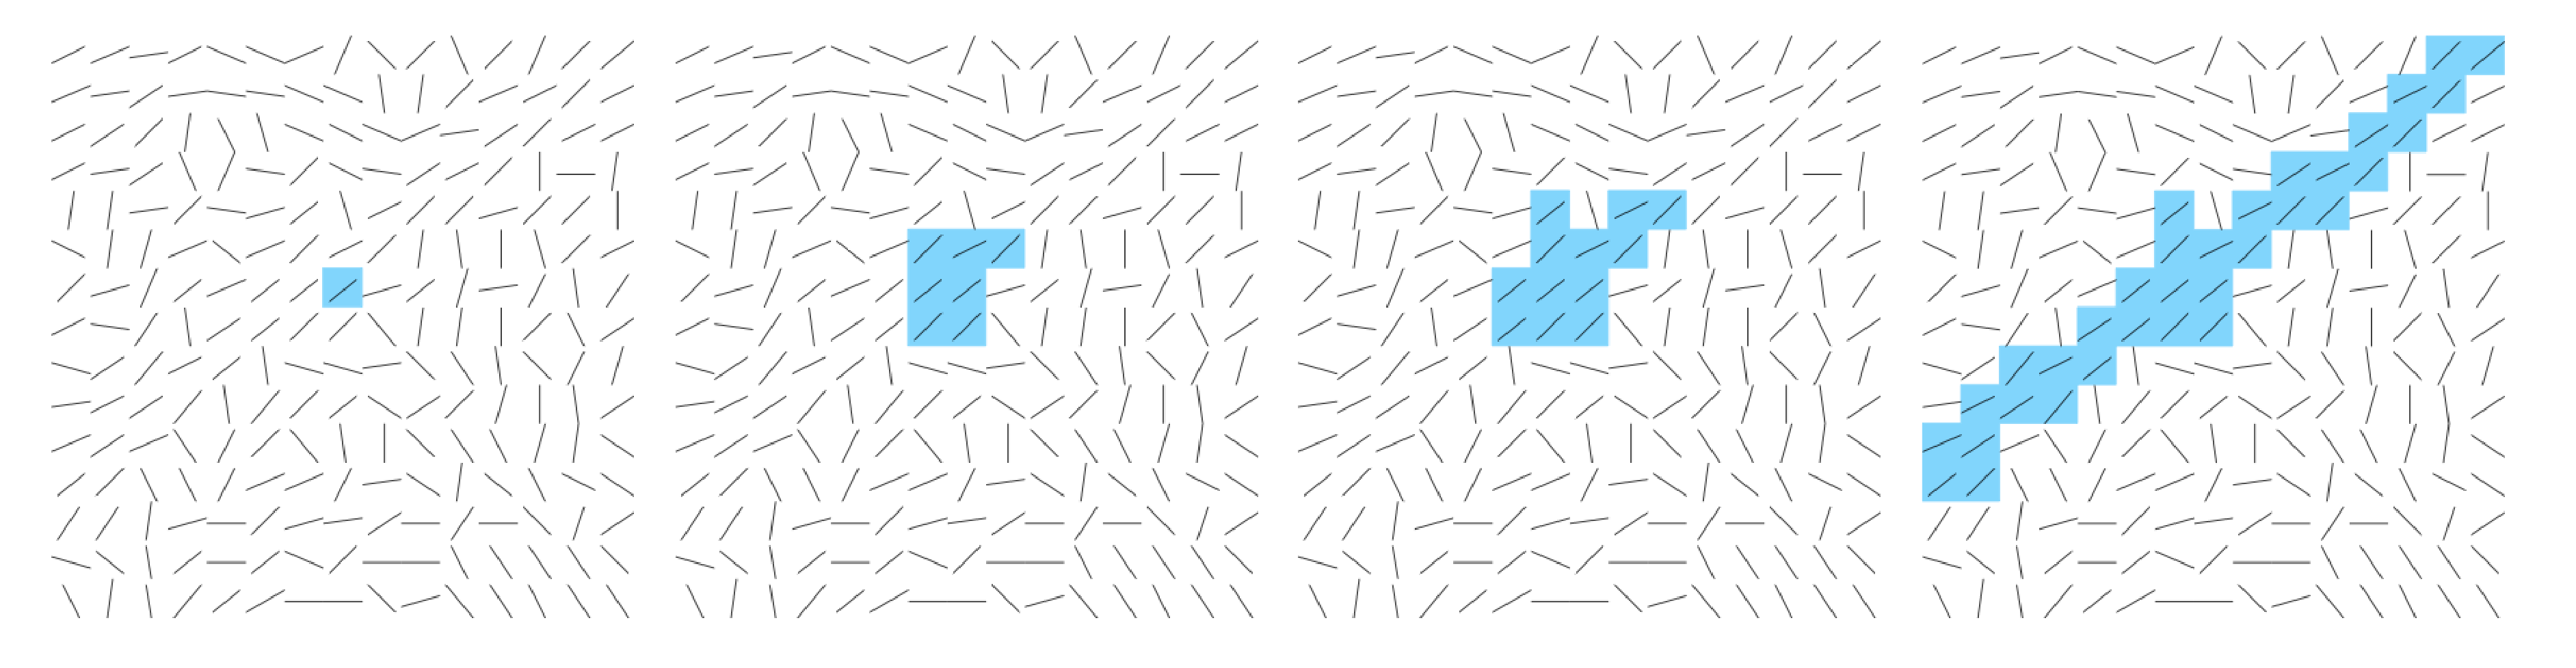
\includegraphics[scale=0.2]{figs_lsd/lsd_1.eps}
\caption{Proceso de crecimiento de una regi�n. El �ngulo asociado cada p�xel de la imagen est� representado por los peque\~nos segmentos y los p�xeles coloreados representan la formaci�n de la regi�n. Tomada de \cite{GJMR12}.}
\label{fig: lsd_1}
\end{figure}

Los p�xels agregados a una regi�n son marcados de manera que no vuelvan a ser testeados. Para mejorar el desempe\~no del algoritmo, las regiones comienzan a evaluarse por los p�xeles con gradientes de mayor amplitud ya que estos representan mejor los bordes. \\

Existen algunos casos puntuales en los que el proceso de b�squeda de \textit{line-support regions} puede arrojar errores. Por ejemplo, cuando se tienen dos segmentos que se juntan y que son colineales a no ser por la tolerancia $\tau$ descripta anteriormente, se detectar�n ambos segmentos como uno solo; ver Figura \ref{fig: lsd_2}. Este potencial problema es heredado del algoritmo de Burns, Hanson y Riseman.

\begin{figure}[h!]
\centering

\includegraphics[scale=0.25]{figs_lsd/lsd_2.eps}
\caption{Potencial problema heredado del algoritmo de Burns, Hanson y Riseman. Izq.: Imagen original. Ctro.: Segmento detectado. Der.: Segmentos que deber�an haberse detectado. Tomada de \cite{GJMR12}.}
\label{fig: lsd_2}
\end{figure}

Sin embargo, LSD plantea un m�todo para solucionar este tipo de problemas. Durante el proceso de crecimiento de las regiones, tambi�n se realiza la aproximaci�n rectangular a dicha regi�n (paso (2) de los tres definidos anteriormente); y si menos de cierto porcentaje umbral de los p�xeles dentro del rect�ngulo corresponden a la \textit{line-support region}, lo que se tiene no es un segmento. Se detiene entonces el crecimiento de la regi�n.

\section{Aproximaci�n de las regiones por rect�ngulos}

\begin{figure}[h!]
\centering
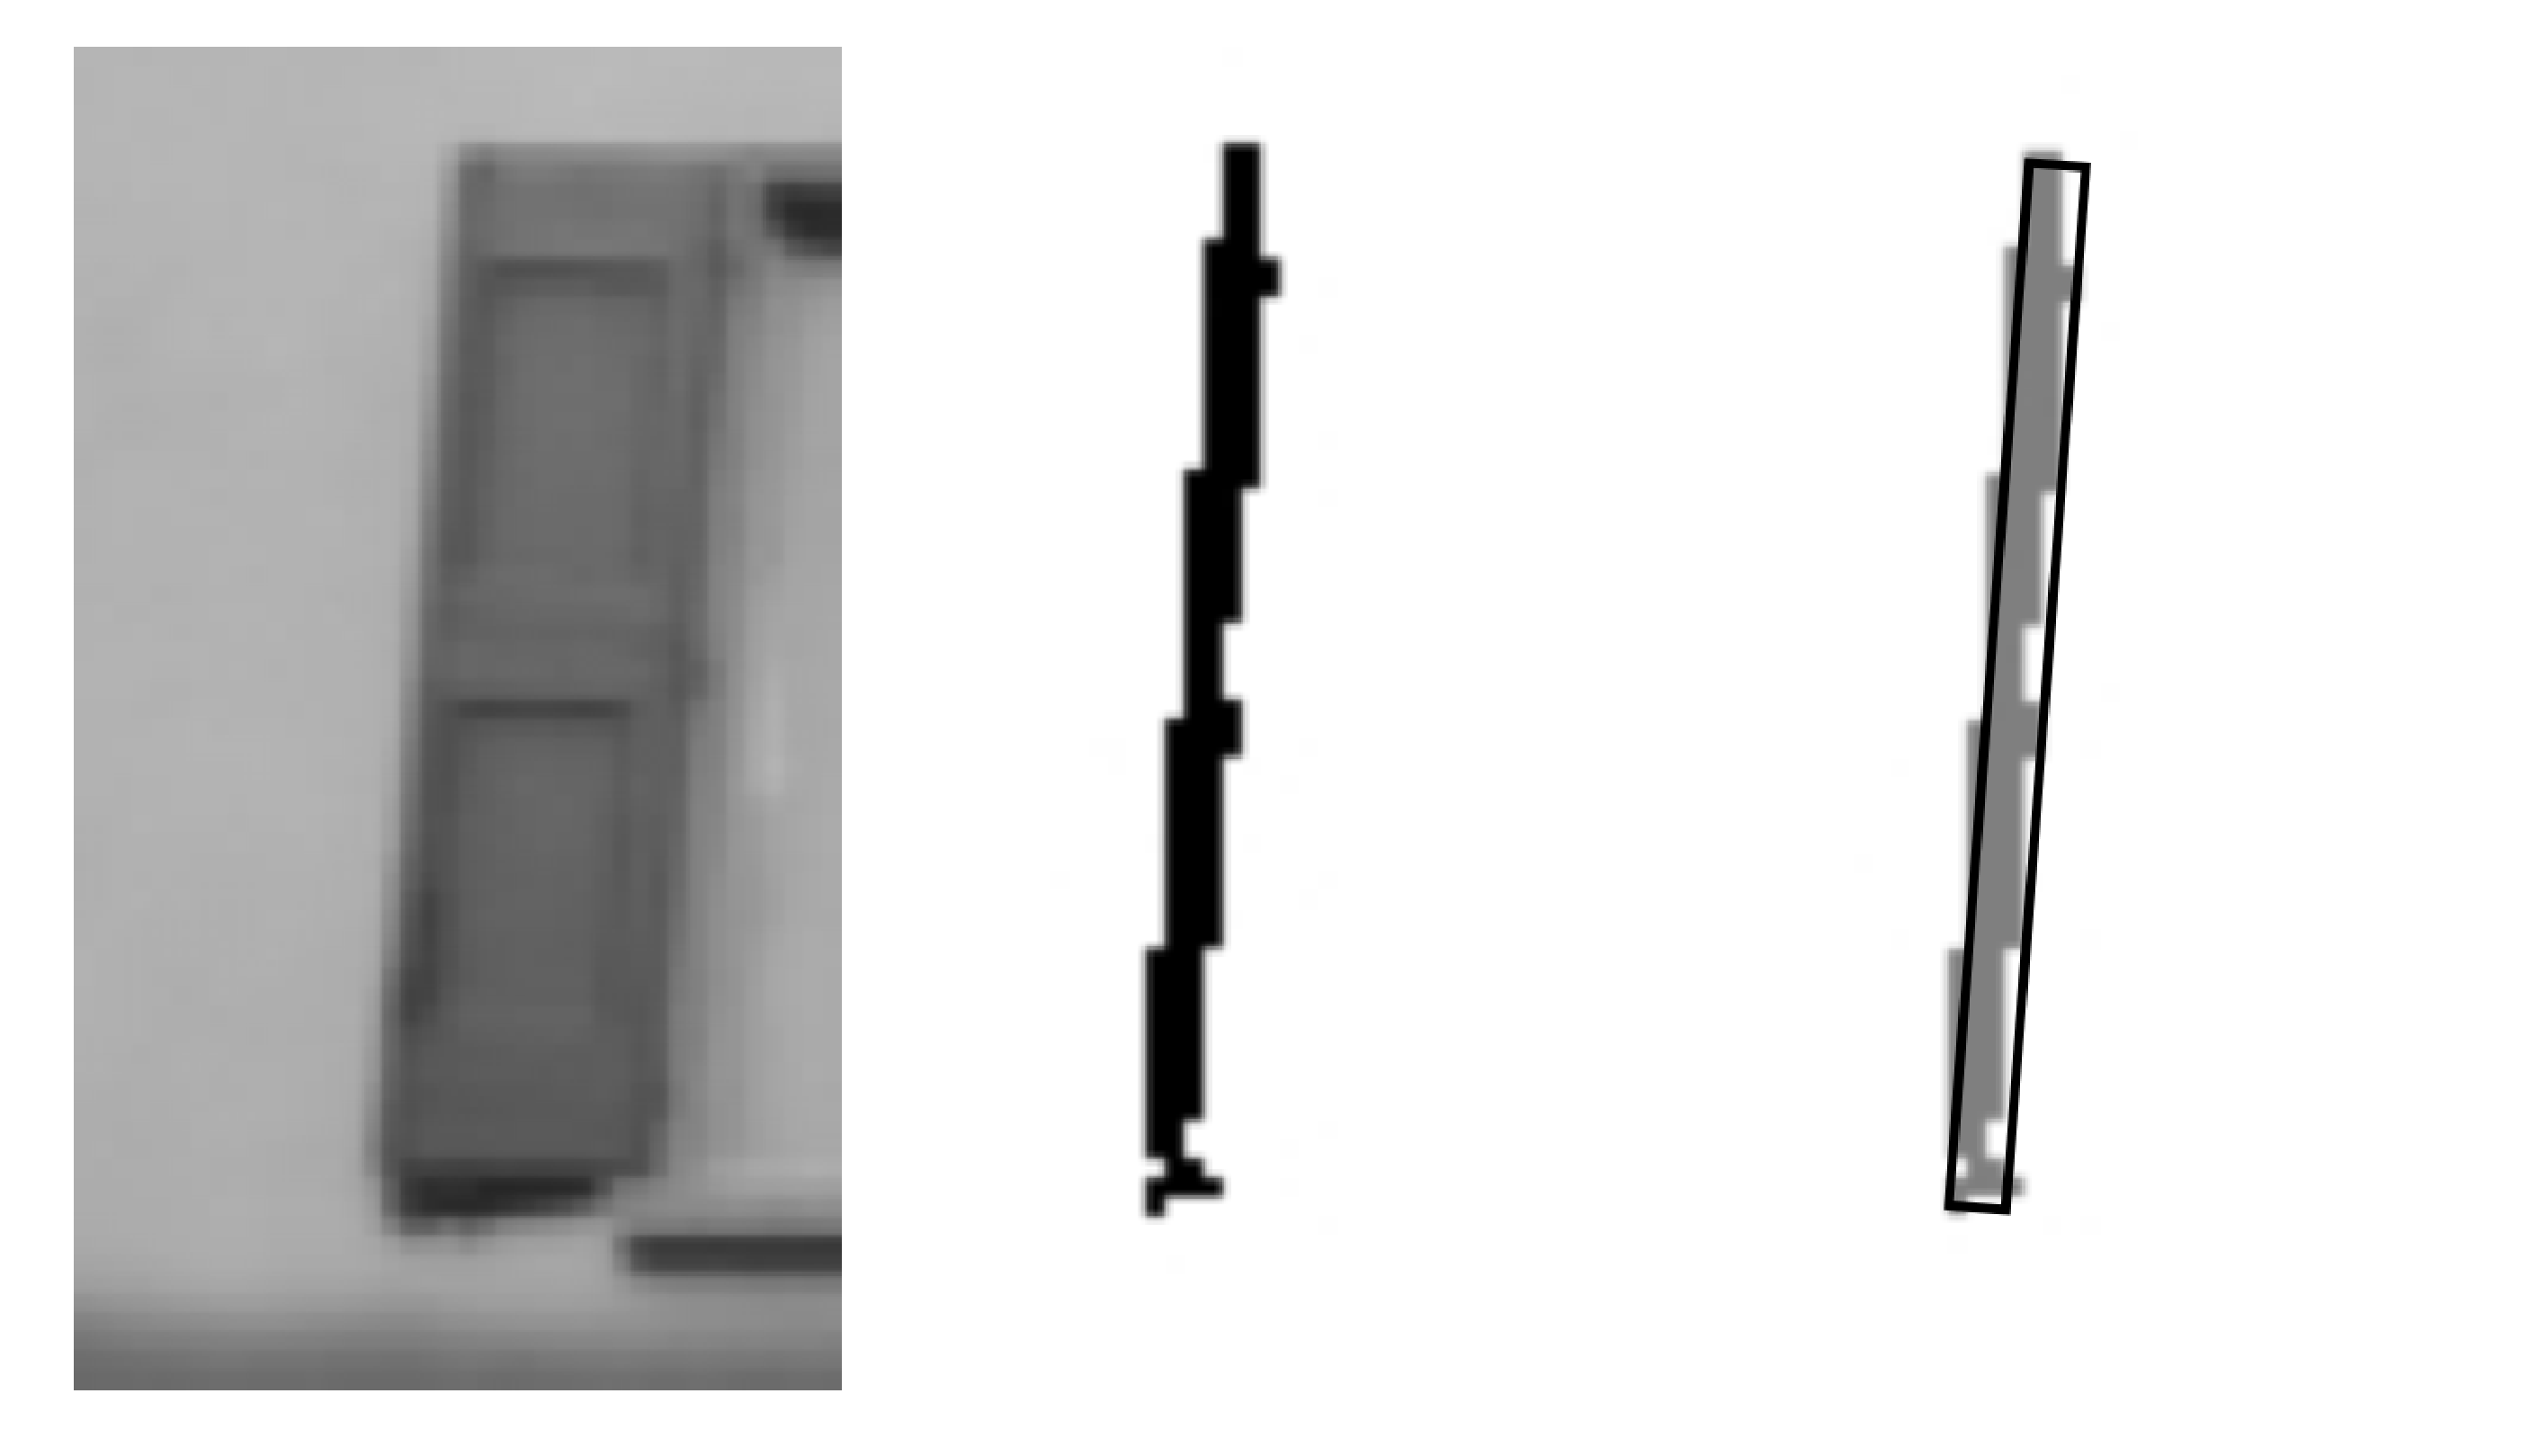
\includegraphics[scale=0.2]{figs_lsd/lsd_3.eps}
\caption{B�squeda del segmento que mejor aproxime cada \textit{line-support region}: aproximaci�n de una regi�n por un rect�ngulo. Izq.: Imagen original. Ctro.: Una de las regiones computadas. Der.: Aproximaci�n rectangular que cubre el $99\%$ de la masa de la regi�n. Tomada de \cite{GJMR12}.}
\label{fig: lsd_3}
\end{figure}

Cada \textit{line-support region} debe ser asociada a un segmento. Cada segmento ser� determinado por su centro, su direcci�n, su anchura y su longitud. A diferencia de lo que pudiese resultar intuitivo, la direcci�n asociada al segmento no se corresponde con la asociada a la regi�n (el promedio de las direcciones de cada uno de los p�xeles). Sin embargo, se elige el centro del segmento como el centro de masa de la regi�n y su direcci�n como el eje de inercia principal de la misma; la magnitud del gradiente asociado a cada p�xel hace las veces de masa. La idea detr�s de este m�todo es que los p�xeles con un gradiente mayor en m�dulo, tienen una mayor probabilidad de corresponder a un borde. La anchura y la longitud del segmento son elegidos de manera de cubir el $99\%$ de la masa de la regi�n.

\section{Validaci�n de segmentos}
La validaci�n de los segmentos previamente detectados se plantea como un m�todo de test de hip�tesis. Se utiliza un modelo \textit{a contrario}. El t�rmino \textit{a contrario} viene del lat�n y significa ``al rev�s'' o ``de forma opuesta''. En procesamiento de im�genes, el principio para la detecci�n \textit{a contrario} define, en primer lugar, un modelo llamado ``\textit{a priori}'' para el caso gen�rico en el que no haya nada que detectar. Entonces la detecci�n de un evento en particular s�lo se dar� cuando la cantidad de ocurrencias de dicho evento en el modelo \textit{a priori} sea lo suficientemente baja. N�tese la aparici�n de cierto valor umbral a ajustar.\\

Para el caso de LSD, dada una imagen de ruido blanco y Gaussiano, se sabe que cualquier tipo de estructura detectada sobre la misma ser� casual. En rigor, se sabe que para cualquier imagen de este tipo, su \textit{level-line orientation field} toma, para cada p�xel, valores independientes y uniformemente distribu�dos entre $[0,2\pi]$. Dado entonces un segmento en la imagen analizada, se estudia la probabilidad de que dicha detecci�n se d� en la imagen de ruido, y si \'esta es lo suficientemente baja, el segmento se considerar� v�lido, de lo contrario se considerar� que se esta bajo la hip�tesis $H_0$: un conjunto aleatorio de p�xeles que casualmente se alinearon de manera de detectar un segmento.\\

Para estudiar la probabilidad de ocurrencia de una cierta detecci�n en la imagen de ruido, se deben tomar en cuenta todos los rect�ngulos potenciales dentro de la misma. Dada una imagen $N\times N$, habr�n $N^4$ orientaciones posibles para los segmentos, $N^2$ puntos de inicio y $N^2$ puntos de fin. Si se consideran $N$ posibles valores para la anchura de los rect�ngulos, se obtienen $N^5$ posibles segmentos. Por su parte, dado cierto rect�ngulo $r$, detectado en la imagen $x$, se denota $k(r,x)$ a la cantidad de p�xeles alineados dentro del mismo. Se define adem�s un valor llamado \textit{Number of False Alarms} (NFA) que est� fuertemente relacionado con la probabilidad de detectar al rect�ngulo en cuesti�n en la imagen de ruido $X$:
\[
NFA(r,x) = N^5. P_{H_0}[k(r,X) \geq k(r,x) ]
\]
v�ase que el valor se logra al multiplicar la probabilidad de que un segmento de la imagen de ruido, de tama\~no igual a $r$, tenga un n�mero mayor o igual de p�xeles alineados que �ste, por la cantidad potencial de segmentos $N^5$. Cuanto menor sea el n�mero NFA, m�s significativo ser� el segmento detectado r; pues tendr� una probabilidad de aparici�n menor en una imagen sin estructuras. De esta manera, se descartar� $H_0$, o lo que es lo mismo, se aceptar� el segmento detectado como v�lido, si y s�lo si:
\[
NFA(r) \leq \epsilon
\] 
donde emp�ricamente $\epsilon=1$ para todos los casos.\\

Si se toma en cuenta que cada p�xel de la imagen ruidosa toma un valor independiente de los dem�s, se concluye que tambi�n lo har�n su gradiente y su \textit{level-line orientation field}. De esta manera, dada una orientaci�n aleatoria cualquiera, la probabilidad de que uno de los p�xeles de la imagen cuente con dicha orientaci�n, a menos de la ya mencionada tolerancia $\tau$, ser�:
\[
p = \frac{\tau}{\pi}
\]
adem�s, se puede modelar la probabilidad de que cierto rect�ngulo en la imagen ruidosa, con cualquier orientaci�n, formado por $n(r)$ p�xeles, cuente con al menos $k(r)$ de ellos alineados, como una distribuci�n binomial:
\[
P_{H_0}[k(r,X) \geq k(r,x) ] = B(n(r), k(r),p).
\]
Finalmente, el valor \textit{Number of False Alarms} ser� calculado para cada segmento detectado en la imgen analizada de la sigiuente manera:
\[
NFA(r,x) = N^5. B(n(r), k(r),p);
\]
si dicho valor es menor o igual a $\epsilon=1$, el segmento se tomar� como v�lido; de lo contrario de dacartar�.

\section{Refinamiento de los candidatos}
Por lo que se vi\'o hasta el momento, la mejor aproximaci\'on rectangular a una \textit{line-support region} es la que obtenga un valor NFA menor. Para los segmentos que no son validados, se prueban algunas variaciones a la aproximaci\'on original con el objetivo de disminu�r su valor NFA y as� entonces validarlos. Esta claro que este paso no es significativo para segmentos largos y bien definidos, ya que estos ser\'an validados en la primera inspecci\'on; sin embargo, ayuda a detectar segmentos m�s peque\~nos y algo ruidosos. \\

Lo que se hace es probar distintos valores para la anchura del segmento y para sus posiciones laterales, ya que estas son los par\'ametros peor estimados en la aproximaci\'on rectangular, pero tienen un efecto muy grande a la hora de validar los segmentos. Es que un error de un p\'ixel en el ancho de un segmento, puede agregar una gran cantidad de p\'ixeles no alineados a este (tantos como el largo del segmento), y esto se ve reflejado en un valor mayor de NFA y puede llevar a una no detecci\'on.\\

Otro m\'etodo para el refinamiento de los candidatos es la disminuci�n de la tolerancia $\tau$. Si los puntos dentro del rect�ngulo efectivamente corresponden a un segmento, aunque la tolerancia disminuya, se computar� pr�cticamente misma cantidad de segmentos alineados; y con una probabilidad menor de ocurrencia ($\frac{\tau}{\pi}$), el valor NFA obtenido ser� menor. Los nuevos valores testeados de tolerancia son: $\frac{\tau}{2}$, $\frac{\tau}{4}$,$\frac{\tau}{8}$,$\frac{\tau}{16}$ y $\frac{\tau}{32}$. El nuevo valor NFA asociado al segmento ser� el menor de todos los calculados.\\  

\section{Optimizaci�n del algoritmo para tiempo real}
Que un algoritmo de procesamiento de im�genes digitales sea temporalmente lineal significa que su tiempo de ejecuci�n crece linealmente con el tama\~no de la imagen en cuesti�n. Estos algoritmos son los mejores para el procesamiento de im�genes en tiempo real. Si bien, como se explic� con anterioridad, los autores de LSD afirman que este es temporalmente lineal; la implementaci�n con la que se cuenta no fue pensada para ser ejecutada en tiempo real. As� entonces, para poder aumentar la tasa de cuadros por segundo total de la aplicaci�n, hubo que realizar algunos cambios m�nimos en el c�digo, simpre buscando que estos alteren lo menos posible el desempe\~no del algoritmo. Se trabaj� sobre ciertos bloques en particular.\\

\subsection{Filtro Gaussiano}
Antes de procesar la imagen con el algoritmo tal y como se vi� en secciones anteriores, la misma es filtrada con un filtro Gaussiano. Se busca en primer lugar, disminuir el tama\~no de la imagen de entrada con el objetivo de disminuir el volumen de informaci�n procesada. Adem�s, al difuminar la imagen, se conservan �nicamente los bordes m�s pronunciados. Para este proyecto en particular, se escogi� la escala del submuestreo fija en $0,5$, un poco m�s adelante en la corriente secci�n se explicar� por qu�.\\

Como la funci�n Gaussiana 2D es separable, el filtrado de la imagen se hace en dos pasos, primero a lo ancho y luego a lo largo. Se utiliza el n�ceo Gaussiano de una dimensi�n normalizado de la Figura \ref{fig: lsd_4}.\\

\begin{figure}[h!]
\centering
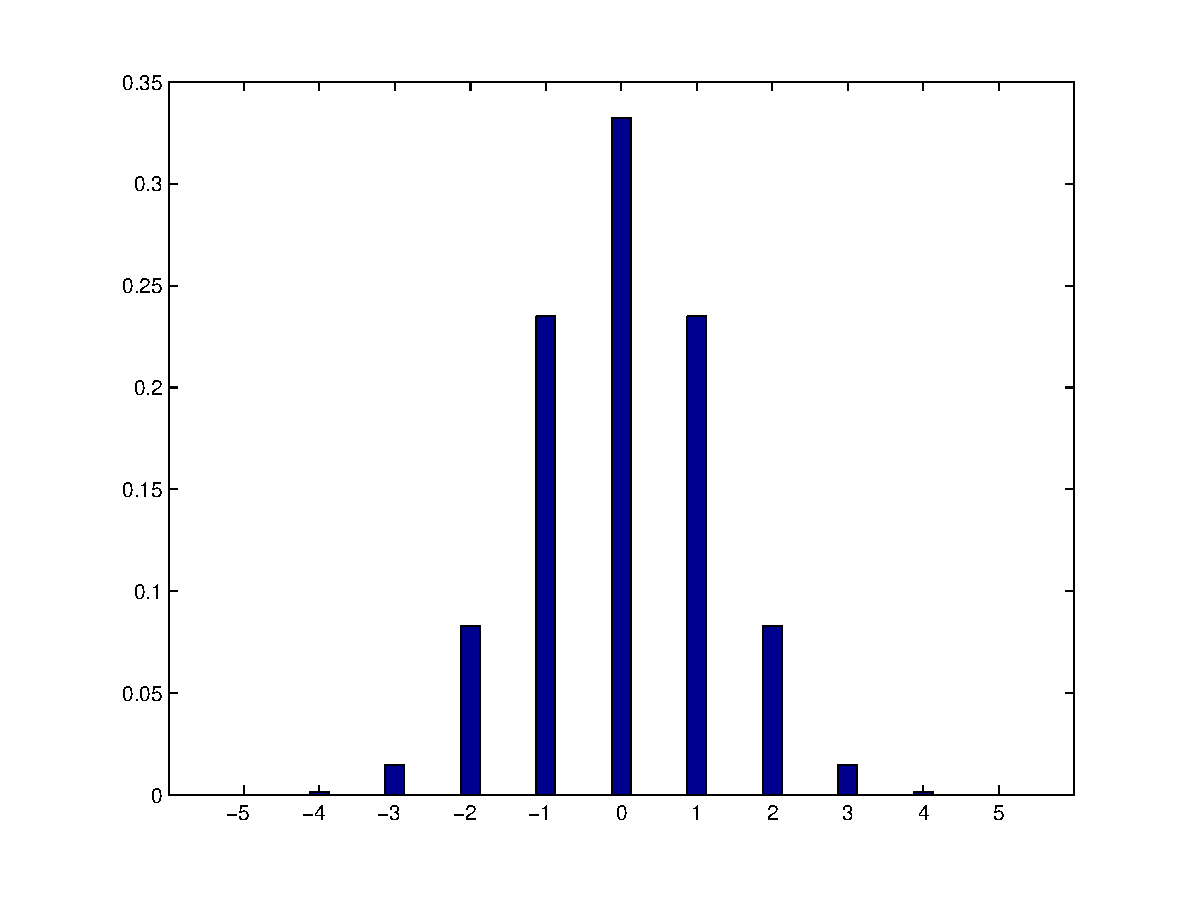
\includegraphics[scale=0.5]{figs_lsd/lsd_4.eps}
\caption{N�cleo Gaussiano utilizado por LSD. $\sigma=1,2$.}
\label{fig: lsd_4}
\end{figure}

De esta manera, se crea una imagen auxiliar vac�a y escalada en $x$ pero no en $y$, y se recorre asign�ndole a cada p�xel en $x$ su valor correspondiente, obtenido del promedio del p�xel $\frac{x}{escala}$ en la imagen original y sus vecinos, todos ponderados por el n�cleo Gaussiano centrado en $\frac{x}{escala}$. Luego se crea otra imagen, pero esta vez escalada tanto en $x$ como en $y$, y se recorre asign�ndole a cada p�xel en $y$ su valor correspondiente, obtenido del promedio del p�xel $\frac{y}{escala}$ en la imagen auxiliar y sus vecinos, todos ponderados por el n�cleo Gaussiano centrado en  $\frac{y}{escala}$. En la Figura \ref{fig: lsd_5} se muestra la relaci�n entre las im�genes.\\

\begin{figure}[h!]
\centering
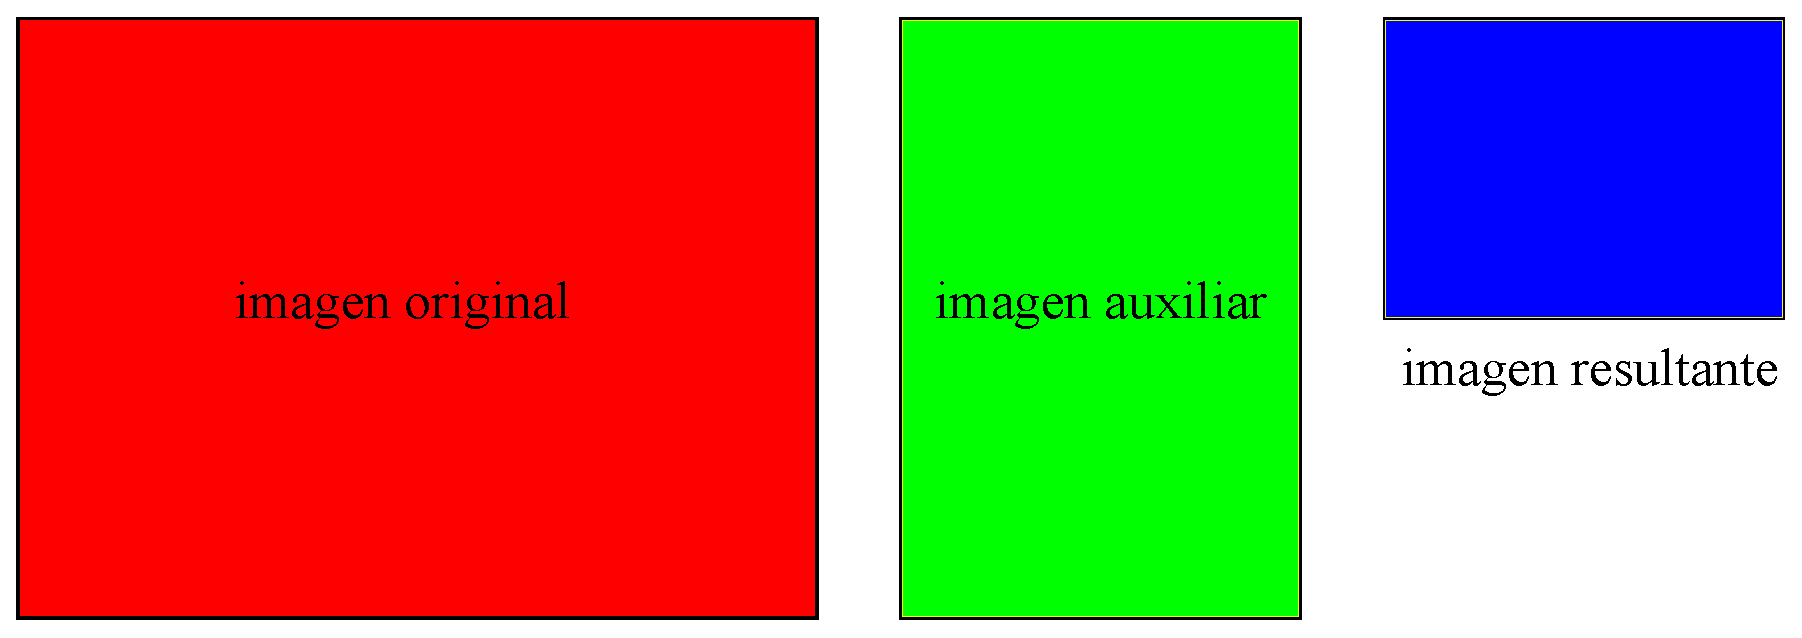
\includegraphics[scale=0.5]{figs_lsd/lsd_5.eps}
\caption{Relaci�n entre las im�genes en consideradas en el filtro Gaussiano. Escala: $0,5$.}
\label{fig: lsd_5}
\end{figure}

V�ase que cuando en el submuestreo $\frac{1}{escala}$ no es un entero, el centro del n�cleo Gaussiano no siempre debe caer justo sobre un p�xel en particular en la imagen original, sino que debe hacerlo entre dos de ellos. Lo que se hace entonces es mover $\pm 0,5$ p�xeles al centro del n�cleo en cada asignaci�n de los p�xeles en las im�genes escaladas; de manera de que la ponderaci�n en el promediado de los p�xeles de la imagen original (y luego la auxiliar) sea la debida. Aunque esta operaci�n le agrega precisi�n al algoritmo, tambi�n le agrega un gran costo computacional, ya que lo que se hace es crear un nuevo n�cleo Gaussiano en cada caso. En particular, para una imagen escalada de $240\times 180$ p�xeles (dimensiones efectivamente utilizadas en este proyecto), debido al filtrado en dos pasos, el n�cleo Gaussiano se crea y se destruye $86400 + 43 200 = 129600$ veces.\\ 

Se decidi� redondear la escala de submuestreo en $0,5$, ya que los valores utlizados emp�ricamente hasta el momento rondaban este valor, y se concluy� que para dicha escala, el n�cleo Gaussiano deb�a permanecer constante, siempre centrado en su sexta muestra (ver Figura \ref{fig: lsd_4}); por lo que se lo quit� de la iteraci�n y actualmente se crea una sola vez al ingresar la imagen al filtro. Es importante destacar que esta optimizaci�n es transparente para el algoritmo si y s�lo si $\frac{1}{escala}=n$, donde $n$ es un entero.\\

Otro cambio que se le realiz� al filtrado Gaussiano fue la supresi�n de las condiciones de borde. Cuando se filtra cualquier imagen con un filtro con memoria, algo importante a tener en cuenta son las condiciones de borde, ya que para el procesamiento de los extremos de la imagen, estos filtros requieren de p�xeles que est�n fuera de sus l�mites. Algunas de las soluciones a este problema son periodizar la imagen, simetrizarla o hasta asumir el valor 0 para los p�xeles que est�n fuera de esta. La opci�n escogida por LSD es la simetrizaci�n. Dem�s est� decir que este proceso requeire de cierto costo computacional extra, por lo que se lo decidi� suprimir. Este costo computacional extra se debe a que el algoritmo encargado del filtrado debe estar en cada bucle pregunt�ndose si es necesario contar con el valor de alg�n p�xel fuera de los l�mites de la imagen, y en ese caso asignarle a dicho p�xel el valor de su correspondiente sim�trico, con eje de simetr�a el borde de la imagen m�s pr�ximo. Actualmente, la imagen escalada no es computada en sus p�xeles terminales; estos son 3 al inicio de cada l�nea o columna y 2 al final de cada una de ellas, irrelevantes en el tama\~no total de la imagen y tambi�n, por ser un filtro FIR (``Finite Impulse Response''), en el resultado del filtrado en general. Ver Figura \ref{fig: lsd_67}.\\

\begin{figure}[h!]
\centering
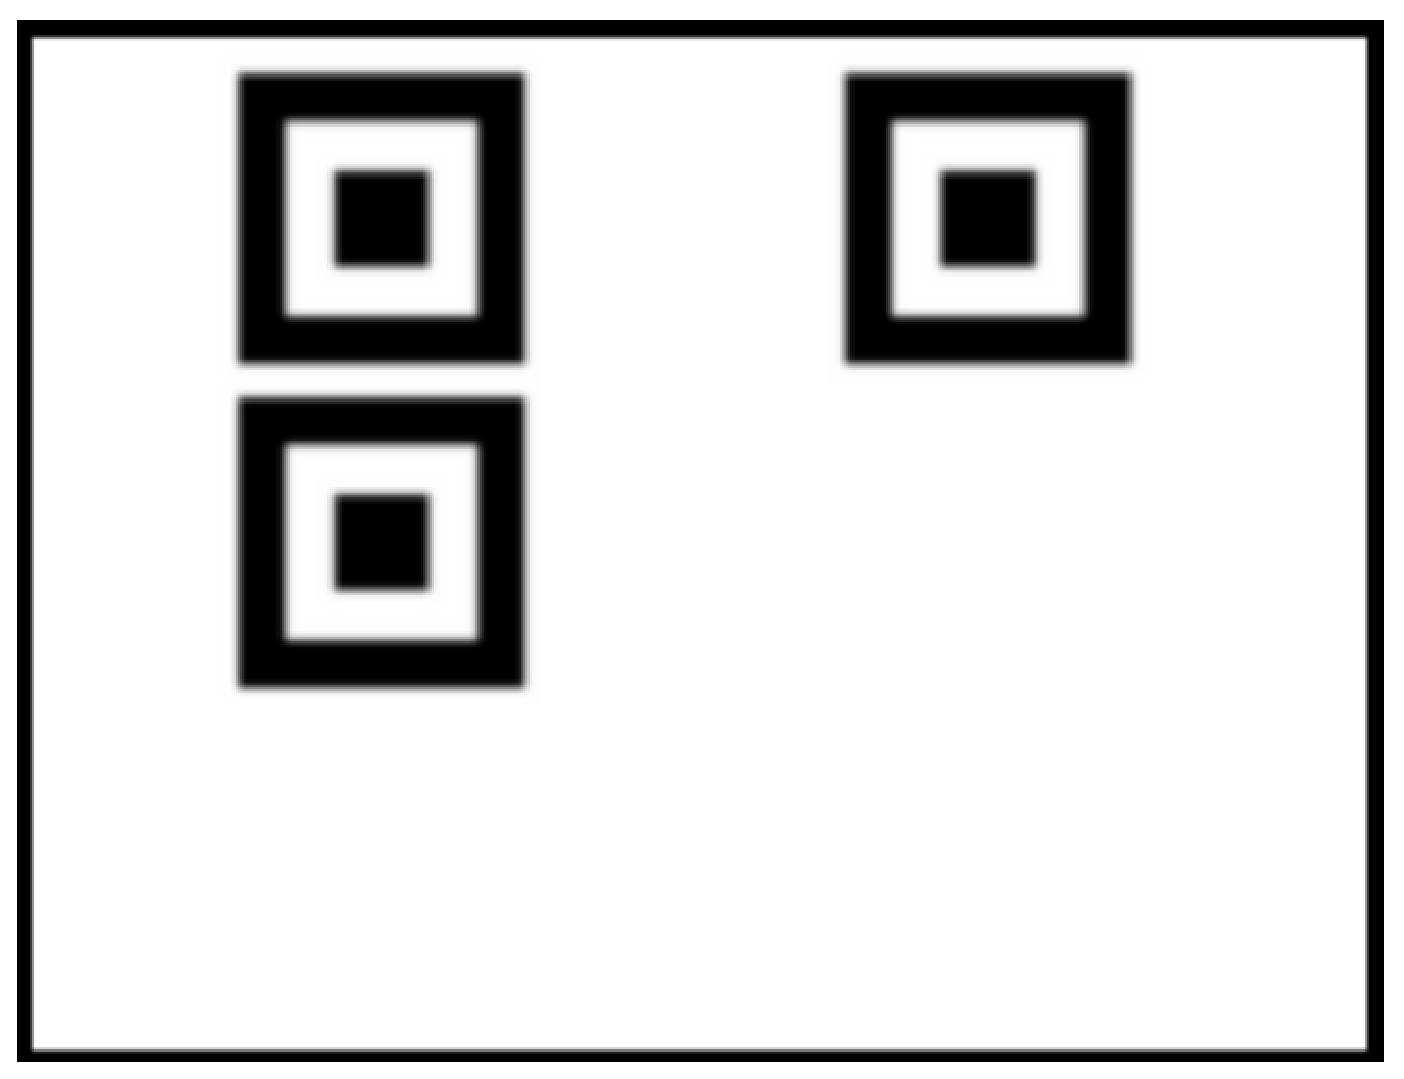
\includegraphics[scale=0.25]{figs_lsd/lsd_6.eps}			

\includegraphics[scale=0.25]{figs_lsd/lsd_7.eps}
\caption{Imagen artificial del marcador trasladado y rotado, filtrada con el filtro Gaussiano. Izq.: Filtro Original. Der.: Filtro sin las condiciones de borde.}
\label{fig: lsd_67}
\end{figure}

\subsection{\textit{Level-line angles}}

La funci�n \textit{ll\_angles} es quien calcula el gradiente de la imagen previamente filtrada para luego obtener el llamado \textit{level-line orientation field}, en donde m�s tarde se hallar�n los candidatos a segmentos. Lo que se hizo en esta funci�n fu� limitar el c�lculo del grandiente a los p�xeles donde la imagen escalada haya sido efectivamente computada. De esta manera se ahorra procesamiento innecesario, adem�s de no detectarse las l�neas negras en el contorno de la imagen (Figura \ref{fig: lsd_67}), que de no ser as� se detectar�an. 

\subsection{Refinamiento y mejora de los candidatos}
Se vi� en la explicaci�n del algoritmo el problema de que si hubiesen dos o m�s segmentos que formen entre ellos �ngulos menores o iguales al valor umbral $\tau$, estos ser�an detectados como uno �nico, heredado del algoritmo de Burns, Hanson y Riseman; y se explic� c�mo, mediante un refinamiento de los segmentos, LSD soluciona este problema. Se vi� adem�s que luego de la validaci�n o no de los segmentos previamente detectados, se realiza una mejora de los mismos para intentar que los no validados a causa de una mala estimaci�n rectangular, s� puedan serlo. \\

Como en este proyecto en particular se trabaja con marcadores formados por cuadrados concentricos, de bordes bien marcados y que forman �ngulos rectos entre s�, el refinamiento y la mejora de los candidatos no es algo que afecte la detecci�n de los mismos; y por consiguiente se suprimieron ambos bloques. Como era de esperarse, dichas supresiones no significaron un cambio considerable en el algoritmo desde el punto de vista del desempe\~o ni del tiempo de ejecuci�n cuando tan s�lo se enfoca al marcador. Sin embargo, si las im�genes capturadas cuentan con muchos segmentos (im�genes naturales gen�ricas), se ve que la detecci�n de los mismos es menos precisa que la del algoritmo original, pero que los tiempos de procesamiento son notablemente inferiores.\\ 

 \subsection{Algoritmo en precisi�n simple}

Originalmente, LSD fue implementado en precisi�n doble o \textit{double} (en general 64 bits por valor). Sin embargo, el \textit{ipad 2} (dispositivo para el cual se optimiz� el algoritmo), cuenta con un procesador \textit{ ARM Cortex-A9}, cuyo bus de datos es de 32 bits. Se decidi� entonces probar cambiar al algoritmo a precisi�n simple o \textit{float} (32 bits por valor) y los resultados fueron realmente buenos. No s�lo el algoritmo baj� su tiempo de ejecuci�n, sino que adem�s no existen cambios notorios en el desempe\~no del mismo.

\subsection{Resultados}

\subsubsection{Filtro Gaussiano}
\begin{figure}[h!]
\centering

\includegraphics[scale=0.25]{figs_lsd/lsd_8.eps}
\caption{Imagen sint\'etica del marcador trasladado y rotado.}
\label{fig: lsd_8}
\end{figure}
Se analizaron los tiempos promedio para la ejecuci�n del filtro Gaussiano original y del optimizado, ambos con precisi�n doble y simple. La imagen de prueba fue la de la Figura \ref{fig: lsd_8}; s�pase que por c�mo es el algoritmo, el contenido de la imagen es independiente del tiempo de procesamiento en cualquiera de los casos, por lo que basta con una �nica imagen de prueba para sacar conslusiones respecto del desempe\~no del mismo. Los valores relevantes del experimento se muestran en las tablas \ref{tab:gaussian_double} y \ref{tab:gaussian_float}:
\begin{itemize}
\item \textbf{Precisi�n doble (\textit{double})}

\begin{table}[h!]
\centering
\begin{tabular}{|c|c|c|} \hline
 														& Filtro original 			& Filtro optimizado \\ \hline
 Tama\~no de imagen	de entrada	& $480\times 360$		&	$480\times 360$	\\ \hline
 Escala												&	$0,5$						&	 	$0,5$				\\ \hline
 Tama\~no de imagen de salida		& $240 \times 180$	& $240 \times 180$ \\ \hline
Segmentos detectados						& $36$							& $36$ \\ \hline
Tiempo medio de procesamiento		& \textbf{36ms}			& \textbf{29ms} \\ \hline
\end{tabular} 
\caption{Comparaci�n entre los tiempos de ejecuci�n del filtro Gaussiano optimizado y el original. Ambos con precisi�n doble.}
\label{tab:gaussian_double}
\end{table}


\item \textbf{Precisi�n simple (\textit{float})}

\begin{table}[h!]
\centering
\begin{tabular}{|c|c|c|} \hline
 														& Filtro original 			& Filtro optimizado \\ \hline
 Tama\~no de imagen	de entrada	& $480\times 360$		&	$480\times 360$	\\ \hline
 Escala												&	$0,5$						&	 	$0,5$				\\ \hline
 Tama\~no de imagen de salida		& $240 \times 180$	& $240 \times 180$ \\ \hline
 Segmentos detectados					& $36$							& $36$ \\ \hline
 Tiempo medio de procesamiento	& \textbf{28ms}				& \textbf{20ms} \\ \hline
\end{tabular} 
\caption{Comparaci�n entre los tiempos de ejecuci�n del filtro Gaussiano optimizado y el original. Ambos con precisi�n simple.}
\label{tab:gaussian_float}
\end{table}

\end{itemize}
\subsubsection{\textit{Line Segment Detection}}
\begin{figure}[h!]
\centering
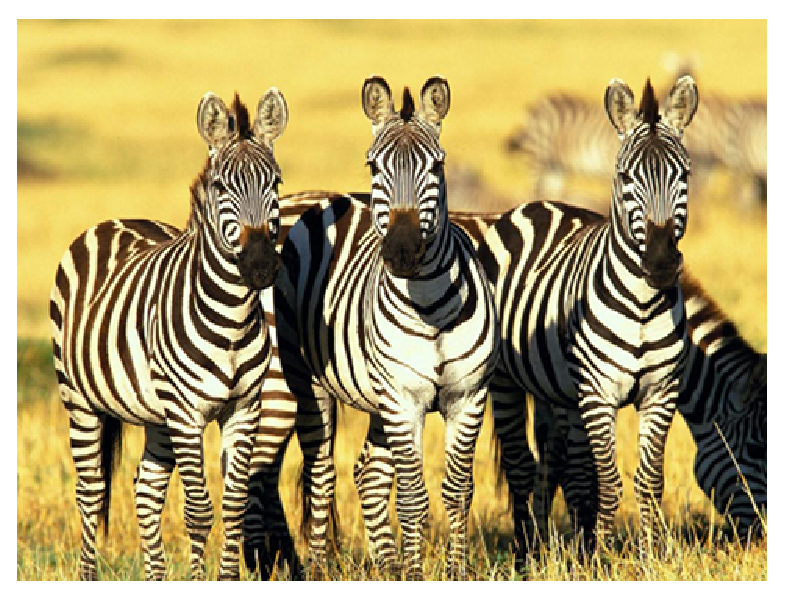
\includegraphics[scale=0.5]{figs_lsd/lsd_9.eps}
\caption{Imagen \textit{zebras.png}.}
\label{fig: lsd_9}
\end{figure}

Se analizaron los tiempos conjuntos para la ejecucici\'on de LSD m\'as el filtro Gaussiano, los originales y los optimizados, ambos con precisi\'on doble y simple. Se probaron ambos bloques juntos ya que el algoritmo original est\'a implementado con \'estos integrados. Las im\'agenes de prueba fueron la del marcador sint\'etico (Figura \ref{fig: lsd_8}) y \textit{zebras.png} mostrada en la Figura \ref{fig: lsd_9}. Los valores relevantes de los experimentos se muestran en las tablas \ref{tab:lsd_double1}, \ref{tab:lsd_double2}, \ref{tab:lsd_float1} y \ref{tab:lsd_float2}.
\begin{itemize}
\item \textbf{Precisi�n doble (\textit{double})}

\begin{table}[h!]
\centering
\begin{tabular}{|c|c|c|} \hline
 														& Algoritmo original 	& Algoritmo optimizado \\ \hline
 Imagen utilizada								& marcador sint\'etico	& marcador sint\'etico \\ \hline
 Tama\~no de imagen	de entrada	& $480\times 360$		&	$480\times 360$	\\ \hline
 Escala												&	$0,5$						&	 	$0,5$				\\ \hline
 Tama\~no de imagen de salida		& $240 \times 180$	& $240 \times 180$ \\ \hline
  Segmentos detectados					& $36$						& $36$ \\ \hline
Tiempo medio de procesamiento		& \textbf{55,4ms}		& \textbf{48ms} \\ \hline
\end{tabular} 
\caption{Comparaci�n entre los tiempos de ejecuci�n del filtro Gaussiano m�s LSD optimizados y los originales, para la imagen \ref{fig: lsd_8}. En todos los casos con precisi�n doble.}
\label{tab:lsd_double1}
\end{table}

\begin{table}[h!]
\centering
\begin{tabular}{|c|c|c|} \hline
 														& Algoritmo original	&	Algoritmo optimizado \\ \hline
Imagen utilizada								& \textit{zebras.png}	& \textit{zebras.png} \\ \hline
Tama\~no de imagen	de entrada	& $480\times 360$		&	$480\times 360$	\\ \hline
Escala												&	$0,5$						&	 	$0,5$				\\ \hline
Tama\~no de imagen de salida		& $240 \times 180$	& $240 \times 180$ \\ \hline
Segmentos detectados						& $251$						& $179$ \\ \hline
Tiempo medio de procesamiento		& \textbf{179,7ms}		& \textbf{94,4ms} \\ \hline
\end{tabular} 
\caption{Comparaci�n entre los tiempos de ejecuci�n del filtro Gaussiano m�s LSD optimizados y los originales, para la imagen \ref{fig: lsd_9}. En todos los casos con precisi�n doble.}
\label{tab:lsd_double2}
\end{table}

\newpage
\item \textbf{Precisi�n simple (\textit{float})}
\begin{table}[h!]
\centering
\begin{tabular}{|c|c|c|} \hline
 														& Algoritmo original	& Algoritmo optimizado \\ \hline
Imagen utilizada								&  marcador sint\'etico &  marcador sint\'etico	\\ \hline
Tama\~no de imagen	de entrada	& $480\times 360$		&	$480\times 360$	\\ \hline
Escala												&	$0,5$						&	 	$0,5$				\\ \hline
Tama\~no de imagen de salida		& $240 \times 180$	& $240 \times 180$ \\ \hline
Segmentos detectados						& $36$						& $36$ \\ \hline
Tiempo medio de procesamiento		& \textbf{47,8ms}		& \textbf{38,8ms} \\ \hline
\end{tabular} 
\caption{Comparaci�n entre los tiempos de ejecuci�n del filtro Gaussiano m�s LSD optimizados y los originales, para la imagen \ref{fig: lsd_8}. En todos los casos con precisi�n simple.}
\label{tab:lsd_float1}
\end{table}


\begin{table}[h!]
\centering
\begin{tabular}{|c|c|c|} \hline
 														& Algoritmo original 	& Algoritmo optimizado \\ \hline
Imagen utilizada								&  \textit{zebras.png} 	&  \textit{zebras.png} \\ \hline
Tama\~no de imagen	de entrada	& $480\times 360$		&	$480\times 360$	\\ \hline
Escala												&	$0,5$						&	 	$0,5$				\\ \hline
Tama\~no de imagen de salida		& $240 \times 180$	& $240 \times 180$ \\ \hline
Segmentos detectados						& $252$						& $182$ \\ \hline 
Tiempo medio de procesamiento		& \textbf{189,8ms}		& \textbf{90,8ms} \\ \hline
\end{tabular} 
\caption{Comparaci�n entre los tiempos de ejecuci�n del filtro Gaussiano m�s LSD optimizados y los originales, para la imagen \ref{fig: lsd_9}. En todos los casos con precisi�n simple.}
\label{tab:lsd_float2}
\end{table}
\end{itemize}

\section{Conslusi�n}
En el presente cap�tulo se vi� en detalle LSD, un algoritmo de detecci�n de segmentos en im�genes que puede ser considerado el estado del arte en su rubro. Luego se afirm� que, si bien sus autores sostienen que el algoritmo es temporalmente lineal, lo que har�a viable su uso en tiempo real; la implementaci�n disponible del mismo, realizada por los propios autores, no est� optimizada para tal caso y por eso hubo que hacerle algunos prque\~nos cambios al c�digo. Dichos cambios lograron mejoras importantes en cuanto al tiempo de procesamiento, manteniendo pr�cticamente invariado su desempe\~no.\\

Los resultados expuestos en las Tablas \ref{tab:gaussian_double} y \ref{tab:gaussian_float} pueden interpretarse como que la decisi�n de cambiar la precisi�n de la implementaci�n del algoritmo de \textit{double} a \textit{float} fue una idea acertada. Por su parte, la lectura de las Tablas \ref{tab:lsd_double1}, \ref{tab:lsd_double2}, \ref{tab:lsd_float1} y \ref{tab:lsd_float2} sugiere que las mejoras en los tiempos de LSD optimizado para el tiempo real, respecto del original, son del �rden de:

$$
\begin{array}{cc}
\textbf{30\% para im�genes con pocos segmentos;} \\
\textbf{50\% para im�genes naturales gen�ricas, con muchos segmentos.}
\end{array}
$$
Cabe aclarar sin embargo, que si bien los resultados cualitativos\footnote{Se entiende por resultados cualitativos a la ejecuci�n de LSD en tiempo real en el \textit{iPad}, imposibles de ilustrar en el presente texto. Ver Secci�n \ref{sec: casoUso1}.} sugieren resultados similares, los resultados cuantitativos fueron logrados con tan s�lo las dos im�genes presentadas anteriormente.\\


Finalmente, en las Figuras \ref{fig: lsd_10} y \ref{fig: lsd_11} se muestan los resultados luego de haber procesado a las Figuras \ref{fig: lsd_8} y \ref{fig: lsd_9} con LSD, primero con la implementaci�n original y luego con la optimizada. Se puede ver, en primer lugar, la gran diferencia que existe entre la cantidad de segmentos detectados en una y otra imagen. Adem�s, se concluye que el desempe\~no de ambas implementaciones es muy similar para el caso de la imagen \textit{zebras.png} e id�ntico para el caso del marcador.\\

\begin{figure}[h!]
\centering
$
\begin{array}{cc}

\includegraphics[scale=0.3]{figs_lsd/marcador_lsd_original.png} & 
\includegraphics[scale=0.3]{figs_lsd/marcador_lsd_optimizado.png}
\end{array}
$
\caption{Resultado de procesar a la Figura \ref{fig: lsd_8} con LSD. Izq.: Implementaci�n original. Der.: Implementaci�n optimizada.}
\label{fig: lsd_10}
\end{figure}


\begin{figure}[h!]
\centering
$
\begin{array}{cc}
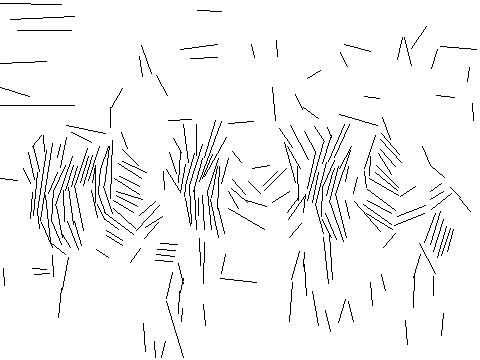
\includegraphics[scale=0.3]{figs_lsd/zebras_lsd_original.png} & 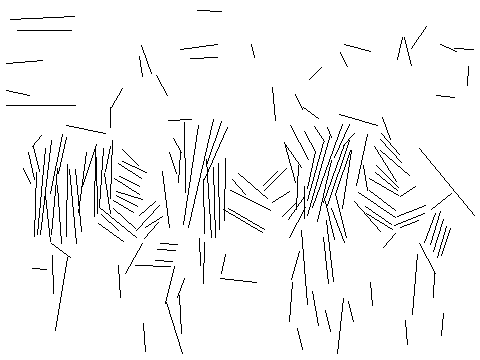
\includegraphics[scale=0.3]{figs_lsd/zebras_lsd_optimizado.png}
\end{array}
$
\caption{Resultado de procesar a la Figura \ref{fig: lsd_9} con LSD. Izq.: Implementaci�n original. Der.: Implementaci�n optimizada.}
\label{fig: lsd_11}
\end{figure}

% Ejemplo de como hacer una cita:
\cite{Daniel03simultaneouspose}.



\bibliographystyle{unsrt}   
\bibliography{encuadro}  
\end{document}
